\chapter{État de l’art}
%https://www.thrillist.com/entertainment/nation/the-netflix-prize


En 2006, la recherche sur les algorithmes de recommandation a suscité beaucoup d’intérêt lorsque Netflix a lancé une compétion le \textbf{« Netflix Prize »} pour améliorer son approche et sa recommandation de films.

\vspace{5mm} 

 A cette époque, l’entreprise est encore un service de location de DVD en ligne mais chaque utilisateur pouvait laisser son avis et attribuer une note entre un et cinq au film. Avant le lancement de cette compétition, Netflix avait déjà son système de recommandation \textbf{« CineMatch »}, permettant de suggérer aux clients un certain nombre de films qu’ils seraient susceptibles d’aimer.
L’intérêt était double pour Netflix, une bonne recommandation fidélise son audience et une récompense d’un million de dollars permet de faire un joli coup de pub au service permettant d’augmenter par la suite son chiffre d’affaires. 

\vspace{5mm} 

L’objectif du concours était de construire un algorithme de recommandation qui pourrait surpasser CineMatch de 10 pourcent. Le concours a suscité beaucoup d’intérêt, tant dans le milieu de la recherche que dans celui des amateurs de films surement grâce à la somme mise en jeu. 

\vspace{5mm} 



\section{Analyse de l'existant }

Le Netflix Prize était une compétition ouverte au public avec la possibilité de participer en équipe ou de façon individuelle. Il n’était pas possible de soumettre son résultat plus d’une fois par jours. Les gagnants du concours ont eu l’obligation de publier leurs résultats ainsi que le code et les licences sur Netflix. Permettant ainsi à Netflix d'exploiter le code de l'équipe gagnante. 


\vspace{5mm} 

Pour la compétition, Netflix a mis à disposition un ensemble de données pour les participants à la compétition. L’ensemble des données contient au total : 

\begin{itemize}
    \item \textbf{480,189 Utilisateurs} : Ce sont des abonnés réels mais ils sont anonymisés.
    \vspace{2mm}
    \item \textbf{17 770 films}.
    \vspace{2mm}
    \item \textbf{Des évaluations de films} allant de 1 à 5.
    \vspace{2mm}
\end{itemize}
\vspace{5mm} 
Le répertoire "training set" contenant 17770 fichiers soit un par film. La première ligne de chaque fichier contient l’identifiant du film ensuite chaque ligne suivante du fichier correspond à une note donnée par un client. Le format de donnée est le suivant : 

\begin{verbatim}
Film X:
Identifiant client, évaluation, date
Identifiant client, évaluation, date
...
\end{verbatim}


Le fichier "qualifying.txt", contient les donneés éligibles pour la compétition. Cet immense fichier est composé d’un identifiant de film et un ensemble de couple <IdentifiantClient, Date> associé au film. L’algorithme rendu doit prévoir toutes les évaluations des clients donnés sur les films dans le jeu de données de qualification en se basant sur les informations disponibles sur chaque utilisateur dans les données "trainning set". Le format des données est le suivant : 
\begin{verbatim}

Identifiant Film 3 :
Identifiant Client 5, date11
Identifiant Client 12, date12


Identifiant Film 4:
Identifiant Client 45, date 11
Identifiant Client 54, date 12
\end{verbatim}

Concernant le format du rendu, il faut remplacer <IdentifiantClient, Date> par la prédiction de note pour le film. Par exemple, si les données du fichier "qualify" sont les suivantes :
\vspace{5mm}

\begin{verbatim}
111:
3245,2005-12-19
5666,2005-12-23
6789,2005-03-14
225:
1234,2005-05-26
3456,2005-11-07
\end{verbatim}
Alors le fichier contenant les prédictions doit ressembler au résultat suivant :
\begin{verbatim}
111:
3.0
3.4
4.0
225:
1,0
2.0
\end{verbatim}
Le résultat 3.0 signifie que le client 3245 évalue le film 111 le 19 décembre 2005 avec la note de 3,0 étoiles.




\vspace{5mm} 

Le dernier fichier donné par Netflix pour réaliser cette compétition est le "probe.txt". Sa structure est la même que le fichier permettant de se qualifier à l'exception qu'il ne contient aucune date (simplement des identifiants de film et de client). Les données contenues dans ce fichier font aussi références aux données dans le répertoire "training set". 

\begin{verbatim}

Identifiant Film 3 :
Identifiant Client 5
Identifiant Client 12


Identifiant Film 4:
Identifiant Client 45
Identifiant Client 54
\end{verbatim}


Netflix fournit aussi un morceau de code permettant de calculer le RMSE\footnote{Le Root Mean Square Error est l'écart type des résidus (erreurs de prédiction).} des prévisions calculées et surtout de comparer cette valeur à celui de Cinematch sur les mêmes données. Pour information, le RMSE de Cinematch est de 0,9514 pour les données fournies. 

%http://www.netflixprize.com/faq#probe pour cette valeur.

\vspace{5mm} 


\section{Comparaison des différentes approches}

Au cours de la compétition, beaucoup d'équipes sont parties sur des approches différentes. 
Trois années après le lancement du « Netflix Prize », le challenge est réussi et remporté par l’équipe "BellKor’s Pragmatic Chaos". Leur solution est un aggrégat de plusieurs algorithmes et de différents modèles mais aussi d'équipes ( BellKor\supercite{BellKor},The Pragmatic Theory\supercite{Pragmatic} et The BigChaos\supercite{BigChaos}). Cette solution fut la première à avoir un meilleur RMSE que cinematch et par consequent à donc remporté la compétition. 


\vspace{5mm}

Durant la compétition, certains algorithmes étaient plus populaires que d'autres et sont  apparus régulièrement. Parmi eux, l’algorithme du plus proche voisin et la factorisation matricielle se sont montrés particulièrement efficace\supercite{LessonsFromNetflixPrize}.

\vspace{5mm}

Une approche via l’algorithme du plus proche voisin (Nearest neighbors) permet de déterminer si deux utilisateurs ont des préférences identiques, proches ou éloignés. Dans le cas du Netflix Prize, les notes attribuées aux différents films permettent de calculer le degré de préférence. Des préférences éloignées ne permettent pas de déterminer les goûts ou notes d’un autre utilisateur. Au contraire des préférences identiques indiquent une relation forte entre deux utilisateurs permettant ainsi de déterminer plus facilement les films à recommander et prédire leur note. Une relation modérée obtenue avec des préférence similaires permet aussi de calculer la note d’un film en fonction d’un delta plus ou moins précis. 

\vspace{5mm}

\begin{figure}[htp]
  \centering
  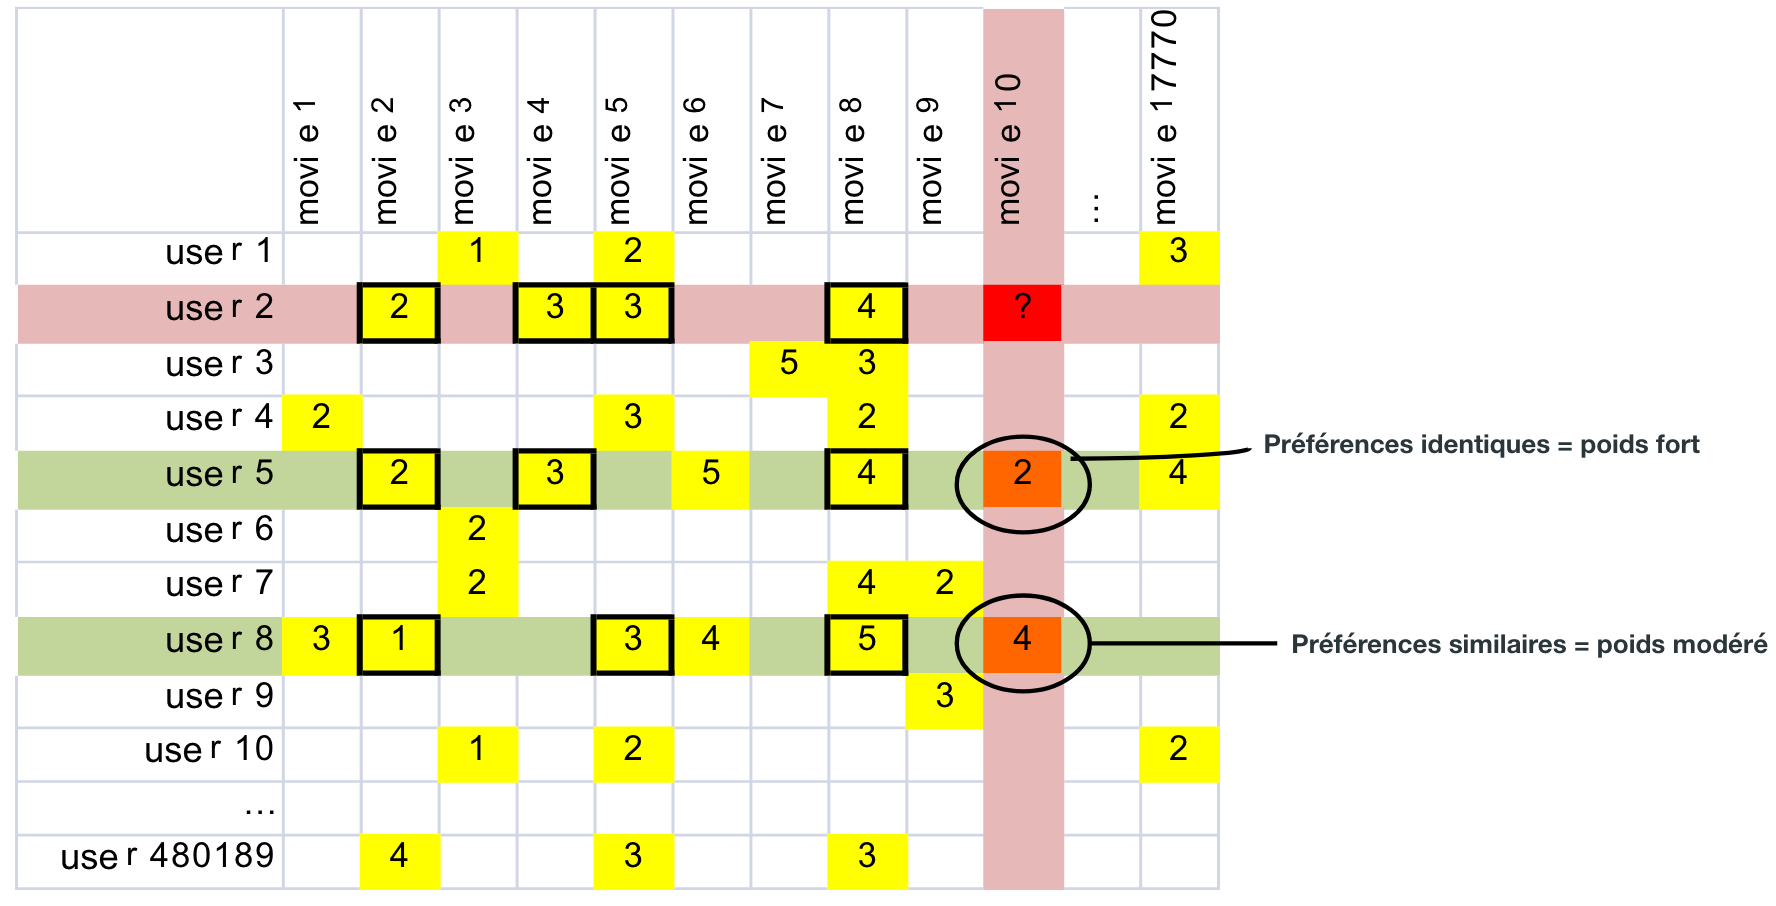
\includegraphics[width=95mm]{./src_img/procheVoisin}
  \caption{Exemple algorithme du plus proche voisin.}
  \label{fig:trois-deux}
\end{figure}

\vspace{5mm}

La factorisation matricielle (Matrix factorization) fait partie des algorithmes de filtrage collaboratif utilisé dans les systèmes de recommandation. Cette approche a prouvé son efficacité au cours du Netflix Prize. Les algorithmes de factorisation matricielle fonctionnent en décomposant la matrice d'interaction "utilisateur-élément" en un produit de deux matrices rectangulaires de plus faibles dimensions. Pour déterminer la note d'un film, il faut alors multiplier et additionner les valeurs pour obtenir la prédiction.

\vspace{5mm}

\begin{figure}[htp]
  \centering
  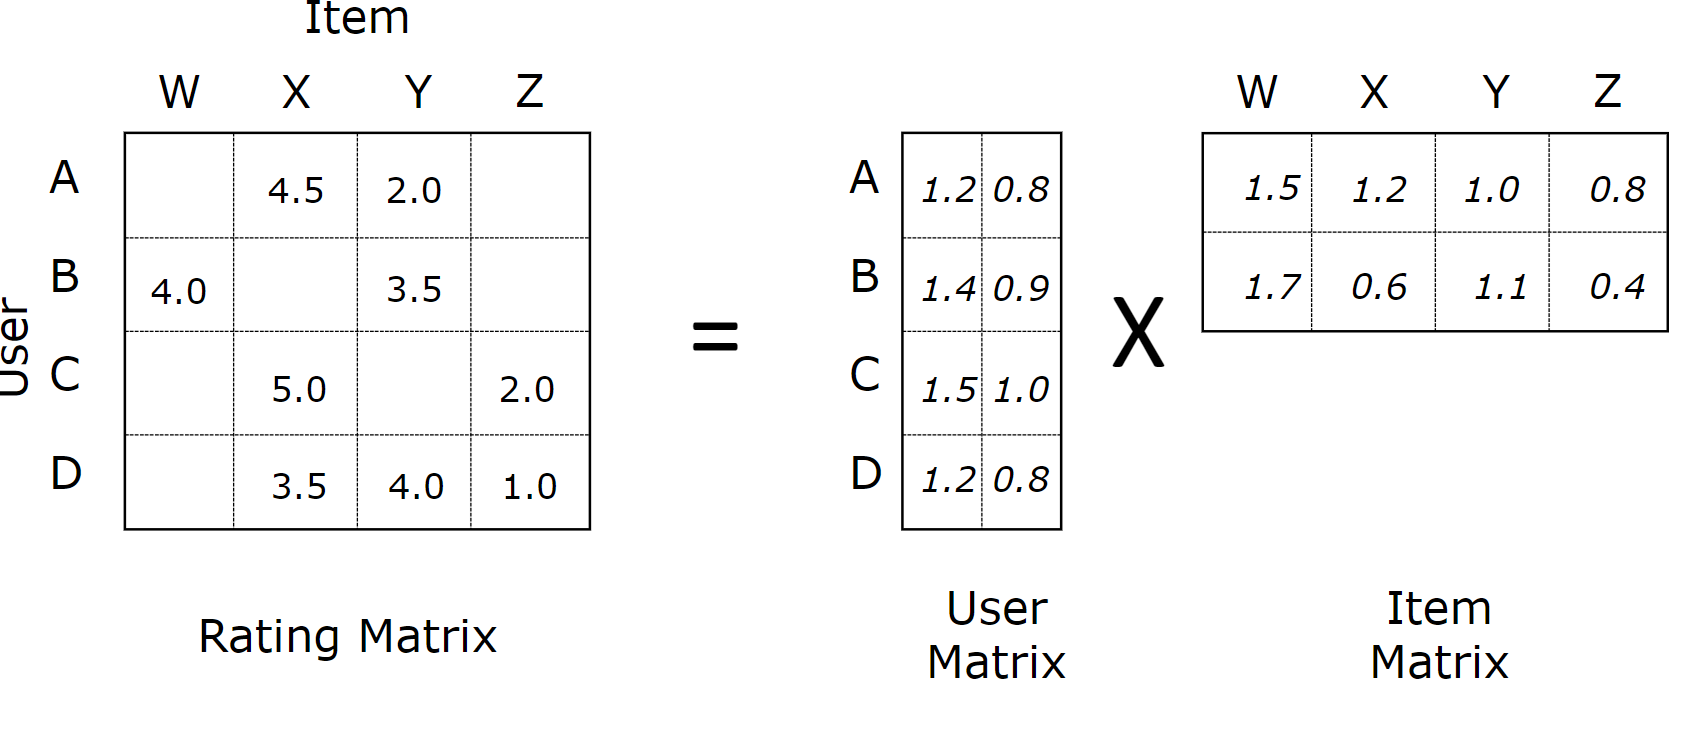
\includegraphics[width=95mm]{./src_img/matrix}
  \caption{Exemple de factorisation matricielle.}
  \label{fig:trois-trois}
\end{figure}

\vspace{5mm}

Ainsi dans l'exemple ci-dessus, la prédiction de l'utisateur A avec l'item W est calculée de la manière suivante : 
\begin{verbatim}

1,2 x 1,5 + 0,8 x 1,7 = 3,16 

\end{verbatim}


L'approche proposée par l’équipe gagnante est articulée autour de 3 axes. Le premier axe modélise les données selon différents niveaux (global, régional et locale). C’est la combinaison de l’extraction des schémas locaux qui sont ensuite factorisés au niveau régional puis affectent globalement les données. Le second axe, est la qualité du modèle, c’est un axe essentiel pour la robustesse permettant la dérivation et les itérations mais aussi d'éviter les effets de débordements lors des factorisations et de l'application d’algorithmes locaux. Afin d’être considérer comme une donnée de qualité et ainsi respecter les critères énoncés il faut que la donnée soit la plus simple possible. Le dernier axe, est une représentation binaire des données selon si les utilisateurs ont donné leur avis de façon implicite ou explicite. Les données sont caractérisées en fonction de leurs évaluations et de la manière dont elles ont été évaluées. Le comportement d’un utilisateur est considéré comme implicite s’il est facile à collecter par son historique de navigation, son historique de location, ses recherches etc... Le retour implicite permet de prédire les évaluations pour les utilisateurs qui n’ont pas encore évalué un film. Quant au retour explicite de l'utilisateur, c'est lorsque ce dernier donne son avis sur le film ou la série par un système de notation (notation du film par une quantité d'étoiles ou bien un symbole de pouce vers le haut ou bien vers le bas). 

\vspace{5mm}

\begin{figure}[htp]
  \centering
  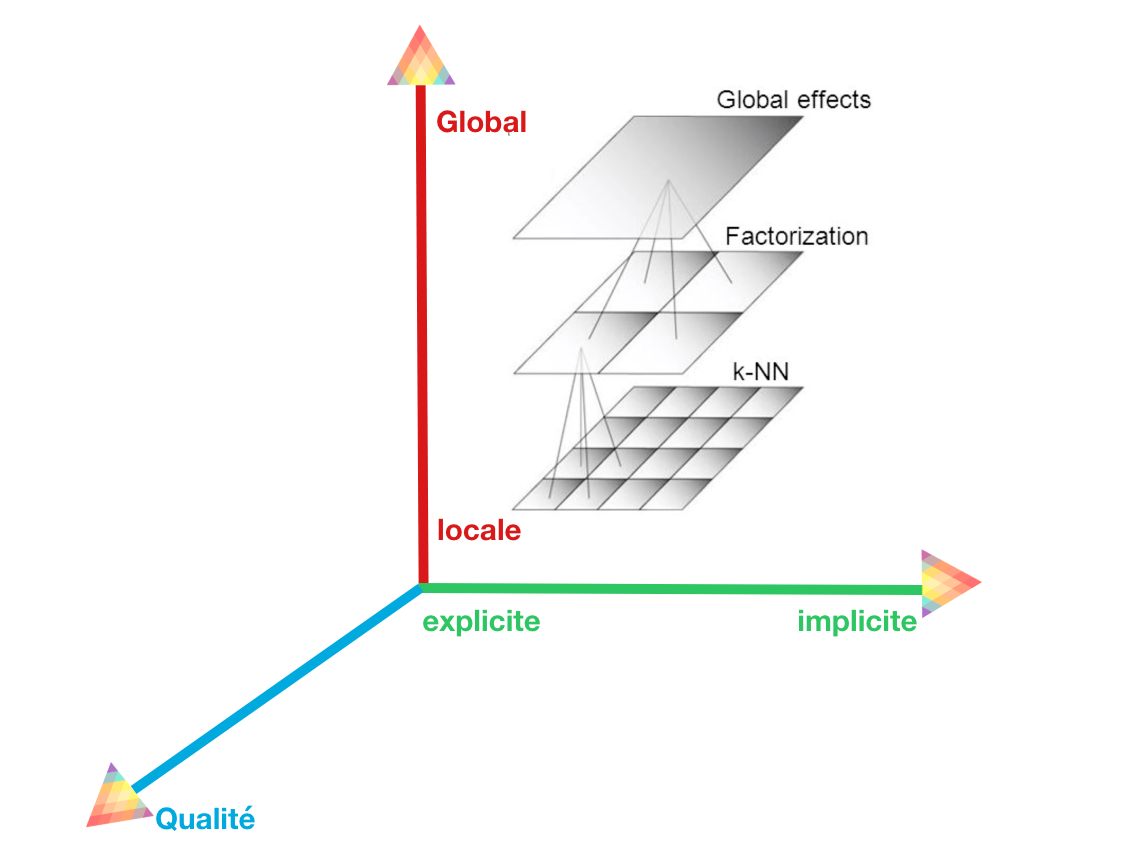
\includegraphics[width=95mm]{./src_img/BPC}
  \caption{Représentation simplifié de la solution BellKor’s Pragmatic Chaos .}
  \label{fig:trois-quatre}
\end{figure}

\vspace{5mm}

%Les solutions proposées sont discutées dans plusieurs articles, notamment [Koren, 2009], [Piotte and Chabbert, 2009] et [Töscher et al., 2009]. Cependant, 

%Malgrès tout le « Netflix Prize » à permis Ce challenge a permis en revanche de mettre en évidence l’intérêt des méthodes de factorisation pour la résolution de problèmes de recommandation, notamment grâce à l’idée d’introduire des informations complémentaires telles que des évaluations implicites, des effets temporels et des niveaux de confiance [Bell and Koren, 2007].
%[Koren, 2009] Koren, Y. (2009). The bellkor solution to the netflix grand prize. Netflix prize documentation, 81.

%[Piotte and Chabbert, 2009] Piotte, M. and Chabbert, M. (2009). The pragmatic theory solution to the netflix grand prize. Netflix prize documentation.

%[Töscher et al., 2009] Töscher, A., Jahrer, M., and Bell, R. M. (2009). The bigchaos solution to the netflix grand prize. Netflix prize documentation, pages 1–52.

%[Bell and Koren, 2007] Bell, R. M. and Koren, Y. (2007). Lessons from the netflix prize challenge. ACM SIGKDD Explorations Newsletter, 9(2) :75–79.

\section{Critique}


Les données mises à disposition pour le Netflix Prize sont issues de réels utilisateurs de Netflix et anonymisées pour des soucis de vie privé. Cependant en 2007, deux chercheurs de l’Université du Texas\supercite{Anonymity} ont réussi à identifier des utilisateurs de façon individuelle par correspondance avec les ensembles de données issues de IMDb\footnote{L’Internet Movie Database (littéralement « Base de données cinématographiques d'Internet »), abrégé en IMDb, est une base de données en ligne sur le cinéma mondial, sur la télévision, et plus secondairement les jeux vidéos.}. 

\vspace{5mm} 

Après une simple étude des données fournies pour réaliser le Netflix Prize, plusieurs choses apparaissent immédiatement comme évidentes. Premièrement, l’ensemble des données fournies est immense avec des variations de notes extrêmes entre les différents utilisateurs. Les variations de note ne permettent pas de déterminer un groupe d’utilisateur semblable facilement. Et deuxièmement, le fichier permettant de s’entrainer et de se qualifier a des propriétés différentes ce qui rajoute une complexité supplémentaire. 

\vspace{5mm} 

Concernant l'utilisation du code de l'équipe gagnante du Netflix Prize,  Xavier Amatriain et Justin Basilico travaillant sur la Science de personnalisation chez Netflix déclarent\supercite{ResultPrize} dans Medium\footnote{Medium est une plateforme web de blog créée en août 2012 par Evan Williams et Biz Stone, les fondateurs de Twitter et Blogger. } : 

\vspace{5mm} 

«A year into the competition, the Korbell team won the first Progress Prize with an 8.43\% improvement. They reported more than 2000 hours of work in order to come up with the final combination of 107 algorithms that gave them this prize. And, they gave us the source code. We looked at the two underlying algorithms with the best performance in the ensemble: Matrix Factorization (which the community generally called SVD, Singular Value Decomposition) and Restricted Boltzmann Machines (RBM). SVD by itself provided a 0.8914 RMSE, while RBM alone provided a competitive but slightly worse 0.8990 RMSE. A linear blend of these two reduced the error to 0.88. To put these algorithms to use, we had to work to overcome some limitations, for instance that they were built to handle 100 million ratings, instead of the more than 5 billion that we have, and that they were not built to adapt as members added more ratings. But once we overcame those challenges, we put the two algorithms into production, where they are still used as part of our recommendation engine.».

\vspace{5mm}

Finalement, même si l'équipe «BellKor's Pragmatic Chaos» a remporté la compétition par un mélange de différents modèles, l'agrégat de plusieurs modèles s'est avéré beaucoup trop coûteux en temps et en énergie pour être mis en place. Dans le reste de l'article, les ingénieures ont mis en avant qu'entre 2006 (date du début de la compétition) et 2009 (fin du concours) les problématiques de Netflix ont changé. Il se pose donc la question de la pertinence d'avoir laissé perdurer cette compétition aussi longtemps. Cependant, selon la citation, les ingénieurs ont déterminé des sous-algorithmes pertinents au sein du travail de l'équipe gagnante. Ce qui a permis d'améliorer les algorithmes de Netflix existants et qui actuellement sont toujours utilisés. 
